\section{Ejercicio IV: Metaheur\'istica}

\subsection{Introducci\'on}

Con el objetivo de mejorar las soluciones obtenidas hasta el momento con las heurísticas constructivas golosas y la de búsqueda local, decidimos implementar una metaheurística GRASP (\textit{Greedy Randomized Adaptatative Search Procedures}), esta es una metaheurística que consiste en construir soluciones iterativamente en base a otras heurísticas quedándose con la mejor de todas las obtenidas. Cada iteración consta fundamentalmente de dos fases una parte constructiva golosa/aleatoria y otra de búsqueda local, esto se repetirá hasta cumplir con un cierto críterio de parada.

\subsection{Algoritmo}

El algoritmo implementando de GRASP consta de un ciclo principal donde en cada iteración construimos una solución factible del problema con una heurística constructiva en base a los parámetros $\alpha$ y $\omega$, estos parámetros indicaran lo golosa o aleatoria que deberá ser la solución, al resultado de la heurística lo refinamos aplicándole búsqueda local considerando una cierta vecindad y comprobamos si el resultado mejoro con respecto a la mejor solución obtenida hasta el momento para conservarla, luego el ciclo se repite si el criterio de parada no fue alcanzado. Inicialmente recibimos como parámetros un criterio de parada del algoritmo, los valores $\alpha$ y $\omega$ y una semilla que usaremos para generar números pseudoaleatorios, en pseudocódigo tenemos lo siguiente:


\begin{algorithm}[H]

\label{}
\caption{Ciclo principal de GRASP}

\begin{algorithmic}[1]

\Statex \underline{Entrada}: Criterio de parada, $\alpha$, $\omega$, semilla
\medskip
\State mejorSoluci\'on $\gets$ $\emptyset$
\While{Criterio de parada no satisfecho}
    \State soluci\'onHeur\'istica $\gets$ ConstruirSoluci\'onHeur\'istica($\alpha$, $\omega$)
	\State soluci\'on $\gets$ AplicarB\'usquedaLocal(soluci\'onHeur\'istica)
	\If{Distancia(soluci\'on) $<$ Distancia(mejorSoluci\'on)}
		\State mejorSoluci\'on $\gets$ soluci\'on
	\EndIf
\EndWhile
\medskip
\Statex \underline{Salida}: mejorSoluci\'on

\end{algorithmic}
\end{algorithm}

La primer fase consiste en armar una solución basada en la heurística del ejercicio 2 pero introduciendo como cambio dos parámetros que indicaran que tan golosa es la elección de elementos. Primero vamos a considerar un camino de todos los gimnasios que tendremos que recorrer, todos estos serán nuestros candidatos a incorporar a la solución y le asignaremos a cada uno de ellos un 'costo incremental' a partir de una evaluación golosa, este costo incremental representa que tanto nos cuesta agregar el elemento a la solución que estamos armando y esta determinado por la distancia del elemento con el último agregado a la lista, inicialmente sera cero si no hay elementos en la lista. Luego a partir de todos nuestros candidatos creamos una nueva lista de candidatos restringidos formada por los mejores candidatos de todos, es decir los que tienen menor costo incremental para incorporarse a la solución (parte golosa del algoritmo), de esta lista de candidatos restringidos tomamos uno al azar (parte probabilística) y lo incorporamos al camino que estamos construyendo y todos los costos incrementales del resto de los candidatos son vueltos a evaluar (parte adaptativa). En pseudocódigo:

\begin{algorithm}[H]

\label{}
\caption{Construir camino de gimnasios}

\begin{algorithmic}[1]

\Statex \underline{Entrada}: $\alpha$
\medskip
\State camino $\gets$ $\emptyset$
\State candidatos $\gets$ gimnasios
\While{Hay gimnasios restantes para agregar al camino}
    \State EvaluarCostos(candidatos)
	\State mejoresCandidatos $\gets$ CandidatosRestringidos(candidatos, $\alpha$)
	\State gimnasio $\gets$ ObtenerGimnasioAleatorio(mejoresCandidatos)
	\State Agregar(gimnasio, camino)
\EndWhile
\medskip
\Statex \underline{Salida}: camino

\end{algorithmic}
\end{algorithm}

Para la elección de los candidatos restringidos vamos a considerar sobre todos los candidatos el valor $costo_{min}$ al que tenga menor costo incremental y $costo_{max}$ al de mayor costo luego la lista restringida esta formada por los candidatos $c$ tal que $costo(c) \in [costo_{min}, costo_{min} + \alpha * (costo_{max} - costo_{min})]$, este intervalo depende del parámetro $\alpha$ donde $\alpha \in [0..1]$. La elección de un $\alpha = 0$ corresponde al intervalo $[costo_{min}, costo_{min}]$ es decir los candidatos serán elegidos de forma puramente golosa mientras que con $\alpha = 1$ el intervalo sera $[costo_{min}, costo_{max}]$ equivalente a una elección puramente aleatoria, luego el parámetro $\alpha$ regula que tan aleatoria o golosa sera la solución en cuestión.

\begin{algorithm}[H]

\label{}
\caption{Candidatos restringidos}

\begin{algorithmic}[1]

\Statex \underline{Entrada}: candidatos, $\alpha$
\medskip
\State costoM\'in $\gets$ CalcularCostoM\'in(candidatos)
\State costoM\'ax $\gets$ CalcularCostoM\'ax(candidatos)
\State candidatosRestringidos $\gets$ $\emptyset$
\For{c : candidatos}
	\If{Costo(c) $\in$ [costoM\'in, costoM\'in + $\alpha$ $\times$ (costoM\'ax - costoM\'in)]}
		\State Agregar(c, candidatosRestringidos)
	\EndIf
\EndFor
\medskip
\Statex \underline{Salida}: candidatosRestringidos

\end{algorithmic}
\end{algorithm}

Con el camino de gimnasios debemos seleccionar las pokeparadas necesarias que debemos visitar para ir recorriendo el camino de gimnasios, para ello vamos a repetir el mismo procedimiento con algunas consideraciones. Primero tomamos el primer gimnasio a recorrer de nuestro camino construido y mientras nos falten pociones para visitarlo vamos a tomar todas las pokeparadas no visitadas como candidatos y le pondremos un costo incremental de la distancia entre esa parada y el gimnasio, nuevamente obtenemos los candidatos restringidos entre todos según el parámetro $\alpha$, y de estos tomamos uno al azar, así hasta recolectar las cantidad de pociones necesarias para visitar al gimnasio y proceder con el siguiente actualizando los costos y volviendo a repetir el ciclo hasta que no queden gimnasios por recorrer. La nueva consideración a tener cuenta es el parámetro $\omega$ que cumple la siguiente función, cuando vamos visitando el camino de gimnasios tomando las pokeparadas necesarias para vencerlo queremos flexibilizar que tanto podemos desviarnos del camino recolectando algunas pociones extra si caben en la mochila, esto representa el parámetro $\omega$ con $\omega \in [0..1]$ la probabilidad de visitar otras paradas adicionalmente de las necesarias, por lo tanto cuando $\omega = 0$ en el camino se recolectaran únicamente las pociones justas para derrotar al gimnasio y pasar al siguiente, cuando $\omega = 1$ siempre se desviara hasta llenar la mochila. Finalmente la construcción de la solución heurística es:

\begin{algorithm}[H]

\label{}
\caption{Construir soluci\'on heur\'istica}

\begin{algorithmic}[1]

\Statex \underline{Entrada}: $\alpha$, $\omega$
\medskip
\State caminoGimnasios $\gets$ ConstruirCaminoGimnasios($\alpha$)
\State soluci\'on $\gets$ $\emptyset$
\State pociones $\gets$ $0$
\State candidatos $\gets$ pokeparadas

\While{Hay gimnasios en caminoGimnasios}
	\While{pociones $<$ Poder(Pr\'ox(caminoGimnasios)) $\lor$ (pociones $<$ mochila $\land$ BoolRnd($\omega$))}
		\State EvaluarCostos(candidatos)
		\State MejoresCandidatos $\gets$ CandidatosRestringidos(candidatos, $\alpha$)
		\State pokeparada $\gets$ ObtenerPokeparadaAleatoria(mejoresCandidatos)
		\State Agregar(pokeparada, soluci\'on)
		\State pociones $\gets$ M\'inimo(pociones$+3$, mochila)
	\EndWhile
	\State pociones $\gets$  pociones $-$ Poder(Pr\'ox(caminoGimnasios))
	\State  Agregar(Pr\'ox(caminoGimnasios), soluci\'on)
	\State  SacarPrimero(caminoGimnasios)
\EndWhile

\medskip
\Statex \underline{Salida}: soluci\'on

\end{algorithmic}
\end{algorithm}

En la segunda fase a esta solución le aplicamos la heurística de búsqueda local implementada eligiendo alguna vecindad. Luego introducimos dos criterios de paradas en el algoritmo:

\paragraph{Criterio I: Iteraciones fijas}
Dado un parámetro $K$ este criterio consiste en interpretar a $K$ como la cantidad de exactas de iteraciones que tendrá el ciclo principal hasta concluir el algoritmo y devolver la solución obtenida.

\paragraph{Criterio II: Iteraciones sin mejoras}
En este criterio de parada es consideramos a $K$ como las iteraciones máximas efectuadas del ciclo sin lograr mejorar la solución obtenida.


\subsection{Complejidad}

Consideramos como parámetros de entrada $G$ cantidad de gimnasios, $P$ cantidad de paradas y $K$ cantidad de iteraciones con el criterio de parada de iteraciones fijas.
El algoritmo consta de un ciclo principal que realiza exactamente $K$ iteraciones en cada iteración llama a una función que construye la solución heurística y luego le aplica búsqueda local esto es \bigo{K  \times  \text{costo(Heurística)}  \times  \text{costo(Búsqueda local)}}. 

Para construir nuestra solución heurística lo primero que realizamos es la construcción de un camino de gimnasios utilizando la función \texttt{graspSolucionGimnasios}, en esta función iteramos sobre la cantidad total de gimnasios y en cada iteración actualizamos todos los gimnasios que son candidatos recorriéndolos todos nuevamente y haciendo operaciones de costo constante como actualizar su costo incremental, luego a estos candidatos los procesamos con la función \texttt{obtenerCandidatosRestringidos} pero esta función tiene costo lineal sobre los candidatos recibidos, por lo tanto todo el costo es de \bigo{G \times (G+G)} $\in$ \bigo{G^2}.

La segunda parte de la heurística se hace llamando a \texttt{graspSolucionAleatoria} en base a un camino de gimnasios de longitud $G$, itera sobre todos los gimnasios del camino y en cada iteración obtiene las paradas que son necesarias visitar el gimnasio actual, la cantidad de paradas que se visitaran entre todos los gimnasios serán como máximo $P$, y en cada parada visitada se actualiza el costo incremental de todas, esto es \bigo{G+P \times P}. Finalmente el costo total de la heurística es de \bigo{G^2+G+P^2} $\in$ \bigo{G^2+P^2}.

Por lo tanto La complejidad temporal de todo el algoritmo es del orden \bigo{K \times (G^2+P^2) \times \text{costo(Búsqueda local)}}.

\subsection{Experimentación}

\subsubsection{Calidad de soluciones}

En este experimento vamos a variar los parámetros $\alpha$ y  $\omega$ sobre una instancia aleatoria de 100 nodos, vamos a correr nuestro algoritmo con un criterio de parada fijo de 100 iteraciones y tomando $\alpha \in [0..1]$ $\omega \in [0..1]$ para comprar la calidad de las soluciones obtenidas, los resultados fueron los siguientes:

\begin{figure}[H]
  \begin{center}
    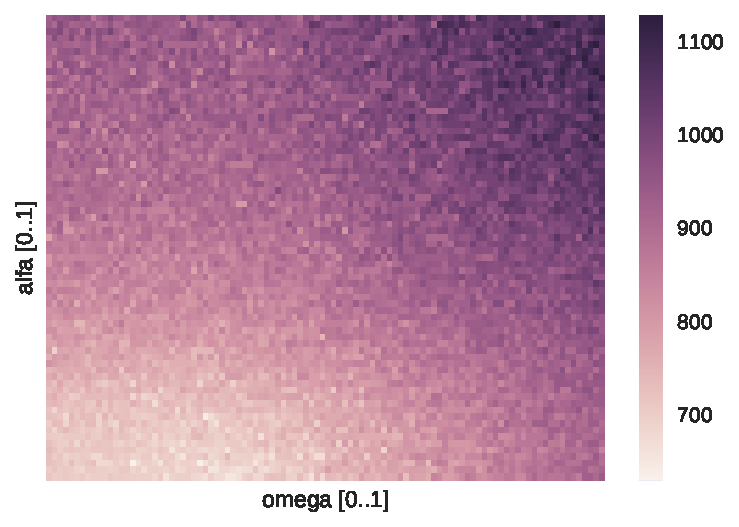
\includegraphics{../experimentacion/ej4/experimento_1.pdf}
    \caption{Mapa de calor en base a las distancias obtenidas.}
    \label{fig:ej3_expAleat_cantCambios}
  \end{center}
\end{figure}

Como podemos ver en este mapa de calor los mejores resultados obtenidos en estas instancias se obtienen fijando valores de $\alpha \in [0.0 ; 0.1]$ y $\omega \in [0.1 ; 0.2]$ es decir tomando soluciones con elecciones bastante golosas pero dándole la oportunidad de realizar pequeños cambios aleatoriamente que resultan en caminos más óptimos, por otro lado permitiendo valores de $\alpha$ y $\omega$ muy altos, es decir permitiendo que elecciones muy aleatorias y permitiendo que se desvíe mucho del camino planteado por la heurística las soluciones empeoran considerablemente.
